\documentclass[10pt]{article}
\usepackage[french]{babel}
\usepackage[utf8]{inputenc}
\usepackage[T1]{fontenc}
\usepackage{amsmath}
\usepackage{amsfonts}
\usepackage{amssymb}
\usepackage[version=4]{mhchem}
\usepackage{stmaryrd}
\usepackage{bbold}
\usepackage{caption}
\usepackage{graphicx}
\usepackage[export]{adjustbox}
\graphicspath{ {./images/} }
\usepackage{eurosym}

\DeclareUnicodeCharacter{20AC}{\ifmmode\text{\euro}\else\euro\fi}

\begin{document}
\captionsetup{singlelinecheck=false}
Nom et prénom :\\
Classe de 1ère : mathématiques spécifiques de l'enseignement scientifique.\\
BAC BLANC

Exercice 1 : QCM sur les automatismes.\\
Pour chacune des trois questions suivantes, une seule réponse est exacte. Laquelle ? L'entourer directement sur cette feuille.

\begin{enumerate}
  \item Augmenter une valeur de $30 \%$ revient à multiplier cette valeur par :\\
a) 0,3\\
b) 0,7\\
c) 1,3\\
d) 1,03
  \item Le prix d'un pantalon a baissé de $20 \%$ en 2025 . Pour retrouver sa valeur initiale, le nouveau prix doit être augmenté de :
\end{enumerate}

\begin{center}
\begin{tabular}{|l|l|l|l|}
\hline
a) $20 \%$ & b) $25 \%$ & c) $30 \%$ & d) $120 \%$ \\
\hline
\end{tabular}
\end{center}

\begin{enumerate}
  \setcounter{enumi}{2}
  \item L'équation $3 x-2=7$ a pour ensemble solution dans $\mathbb{R}$ :\\
a) $S=\{6\}$\\
b) $S=\{3\}$\\
c) $S=\left\{\frac{5}{3}\right\}$\\
d) $S=\{-3\}$
  \item L'expression affine $\mathrm{A}(x)=-3 x+6$ a pour tableau de signes :
\end{enumerate}

\begin{table}[h]
\begin{center}
\captionsetup{labelformat=empty}
\caption{a)}
\begin{tabular}{|c|cccc|}
\hline
$x$ & $-\infty$ &  & 2 & $+\infty$ \\
\hline
$A(x)$ &  & + & 0 & - \\
\hline
\end{tabular}
\end{center}
\end{table}

\begin{table}[h]
\begin{center}
\captionsetup{labelformat=empty}
\caption{b)}
\begin{tabular}{|r|rrrrr|}
\hline
$x$ & $-\infty$ &  & 2 &  & $+\infty$ \\
\hline
$A(x)$ &  & - & 0 & + &  \\
\hline
\end{tabular}
\end{center}
\end{table}

\begin{table}[h]
\begin{center}
\captionsetup{labelformat=empty}
\caption{c)}
\begin{tabular}{|c|ccccc|}
\hline
$x$ & $-\infty$ &  & -2 &  & $+\infty$ \\
\hline
$A(x)$ &  & + & 0 & - &  \\
\hline
\end{tabular}
\end{center}
\end{table}

\begin{table}[h]
\begin{center}
\captionsetup{labelformat=empty}
\caption{d)}
\begin{tabular}{|r|rrrrr|}
\hline
$x$ & $-\infty$ & -2 & $+\infty$ & $+\infty$ &  \\
\hline
$A(x)$ &  & - & 0 & + &  \\
\hline
\end{tabular}
\end{center}
\end{table}

\begin{enumerate}
  \setcounter{enumi}{4}
  \item La forme factorisée de l'expression algébrique $f(x)=x-8 x^{2}$ est :\\
a) $f(x)=x(-8 x)$\\
b) $f(x)=-7 x^{2}$\\
c) $f(x)=-7 x$\\
d) $f(x)=x(1-8 x)$
  \item L'ensemble des solution de l'équation $(x-9)(2 x+3)=0$ est :\\
a) $\left\{9 ;-\frac{3}{2}\right\}$\\
b) $\{9$; 1,5\}\\
c) $\left\{-9 ;-\frac{3}{2}\right\}$\\
d) $\{-9 ; 1,5\}$
\end{enumerate}

\section*{Exercice 2}
On s'intéresse à la population d'une ville. En 2024, la population de la ville était de 15000 habitants. En 2025 cette population a augmenté de 1000 habitants.\\
On fait l'hypothèse que le nombre d'habitants continue d'augmenter de 1000 habitants par an. Pout tout entier naturel $n$, on note $u(n)$ la population de cette ville pour l'année $2024+n$

\begin{enumerate}
  \item Compléter directement sur cette feuille : $u(0)=$ $\_\_\_\_$
  \item Calculer $u(1)$ et écrire une phrase qui explique ce que représente $u(1)$
  \item a) Donner la relation de récurrence de la suite $u$ qui exprime, pour tout entier naturel $n, u(n+1)$ en fonction de $u(n)$\\
b) En déduire la nature de cette suite.
  \item En déduire l'expression, pour tout entier naturel $n$, de $u(n)$ en fonction de $n$
  \item En déduire la population de la ville en 2030 que l'on peut estimer avec ce modèle.
  \item Compléter l'algorithme ci-dessous (directement sur le sujet) afin qu'il affiche au bout de combien d'années la population de cette ville devient supérieure ou égal à 30000 habitants.\\
(Toujours en utilisant le même modèle d'évolution de population)
\end{enumerate}

\begin{verbatim}
$N=0$
$U=15000$
while $U$
    $U=$
    $N=N+1$
print(N)
\end{verbatim}

\section*{Exercice 3}
Sujet E3C 1ST subjectWorkingBlob2189584967921612103\\
Une usine d'horlogerie fabrique une série de montres. Au cours de la fabrication, il apparaît deux types de défauts, le défaut mécanique A et le défaut esthétique B .

Sur un lot de 200 montres, $2 \%$ des montres fabriquées présentent le défaut $\mathrm{A}, 10 \%$ le défaut B et 178 montres ne présentent aucun des deux défauts.

\begin{enumerate}
  \item a. Combien de montres fabriquées présentent le défaut A ?\\
b. Combien de montres fabriquées présentent le défaut B ?\\
c. Recopier et compléter sur votre copie le tableau croisé des effectifs suivant :
\end{enumerate}

\begin{center}
\begin{tabular}{|l|l|l|l|}
\hline
Nombre de montres & Présentant le défaut A & Ne présentant pas le défaut A & Total \\
\hline
Présentant le défaut B &  &  &  \\
\hline
Ne présentant pas le défaut B &  &  &  \\
\hline
Total &  &  & 200 \\
\hline
\end{tabular}
\end{center}

\begin{enumerate}
  \setcounter{enumi}{1}
  \item a. Quelle est la fréquence $f$ des montres présentant les deux défauts ?\\
b. Parmi les montres présentant le défaut B, quel est le pourcentage de celles présentant le défaut $A$ ?\\
c. Le directeur de l'usine affirme : « II y a plus de $90 \%$ des montres qui ne présentent aucun des deux défauts ». A-t-il raison?
\end{enumerate}

\section*{Exercice 4}
L'offre et la demande désignent respectivement la quantité d'un bien ou d'un service que les acteurs du marché sont prêts à vendre ou à acheter à un prix donné.\\
Une étude de marché a permis d'établir que la fonction $f$ représentée ci-dessous, modélise l'offre d'un produit. Elle a également permis de modéliser la demande de ce même produit par la fonction affine $g$ définie, pour tout réel $x \in[1 ; 21], g(x)=-4 x+84$

\begin{itemize}
  \item L'offre $f(x)$ est la quantité, exprimée en milliers d'articles, que les producteurs sont prêts à vendre au prix unitaire de $x$ euros ;
  \item La demande $g(x)$ est la quantité, exprimée en milliers d'articles, que les consommateurs sont prêts à acheter au prix unitaire de $x$ euros.\\
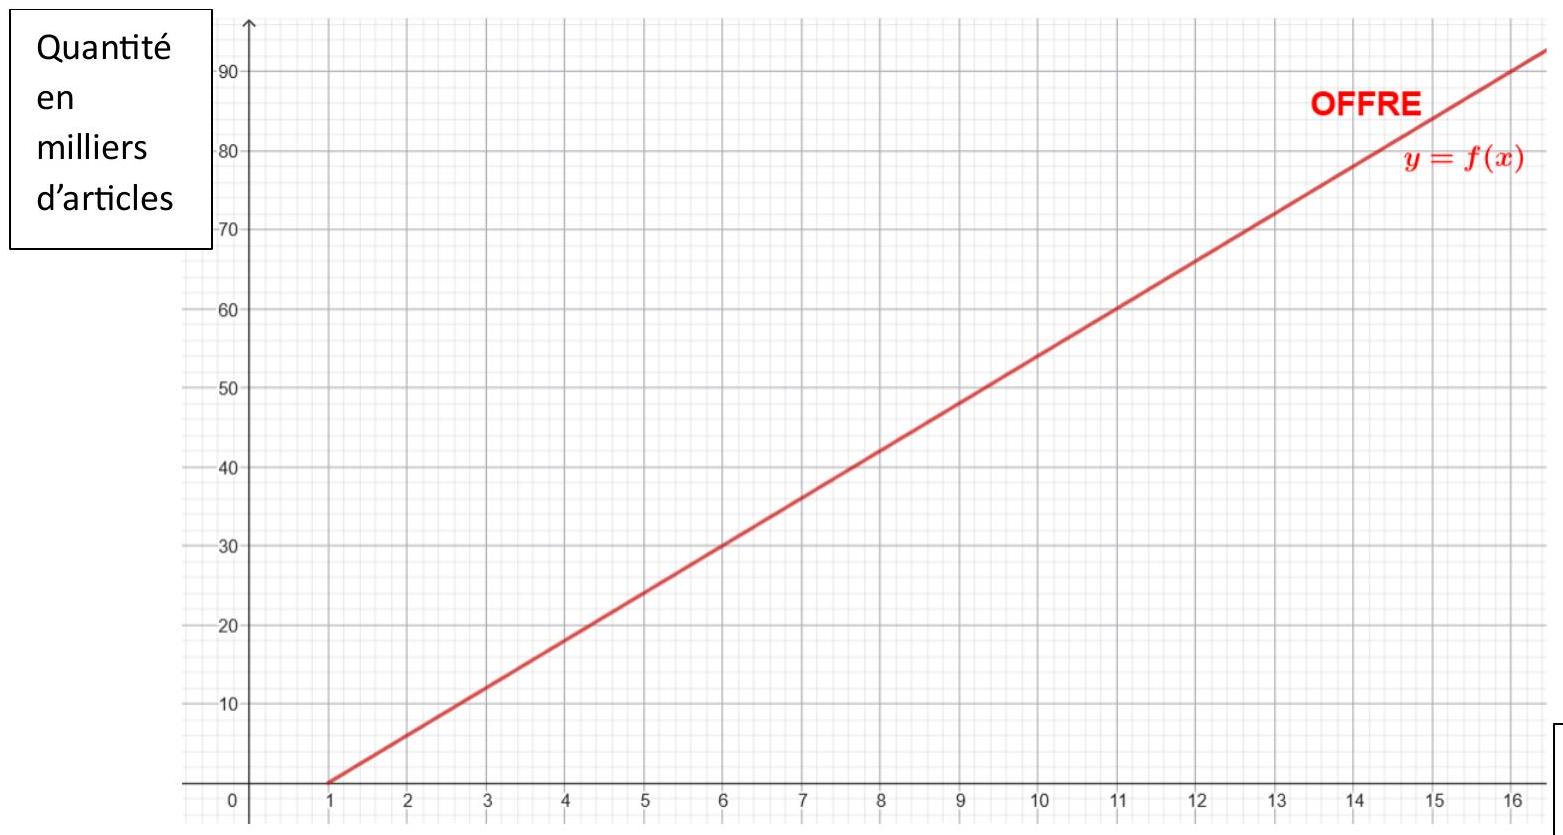
\includegraphics[max width=\textwidth, center]{5fdcb776-ceff-468e-a664-aa6338a4f0b7-3_835_1563_625_169}
\end{itemize}

Prix de vente en €

\begin{enumerate}
  \item On rappelle que la fonction « demande» est définie sur [1; 21] par $g(x)=-4 x+84$\\
a) Pour un prix de vente de $1 €$ à combien d'article correspond la demande des consommateurs ?\\
b) Calculer $g(6)$. Que représente ce résultat ?\\
c) Sur le graphique ci-dessus et à l'aide des calculs précédents, tracer la représentation graphique de la fonction « demande » $g$.
  \item On rappelle que la fonction affine « offre» $f$ définie sur $[1 ; 21]$ est représentée en rouge sur le graphique ci-dessus.\\
a) Lire graphiquement et compléter la réponse directement sur cette feuille $f(1)=$ $\_\_\_\_$\\
b) Pour cette question seulement on considère que le prix de vente est fixé à $6 €$.
\end{enumerate}

Graphiquement déterminer la quantité offerte par les producteurs.\\
c) Déterminer le coefficient directeur de la droite représentant la fonction «offre».

On justifiera à l'aide d'une formule.\\
d) Déterminer l'expression de la fonction $f$.\\
3) a) Résoudre $6 x-6=-4 x+84$\\
b) On dit que le marché est à l'équilibre lorsque, pour un même prix, la quantité offerte est égale à la quantité demandée.\\
En déduire le prix d'équilibre et la quantité associée.


\end{document}